\documentclass{article}

% chinese fonts
\usepackage{ctex}

% math fonts
\usepackage{amsmath}
\usepackage{amsthm}
\usepackage{amssymb}
\usepackage{bm}

% figures
\usepackage{tikz}
\usepackage{graphicx}
\graphicspath{{./figures/}}

% tables
\usepackage{tabularx}
\usepackage{booktabs}
\usepackage{multirow}

% codes
\usepackage{listings}
\lstset{language     = Matlab,
        basicstyle   = \ttfamily,
        keywordstyle = \color{cyan},
        rulecolor    = \color{black},
        commentstyle = \color{green},
        keepspaces   = true,
        tabsize      = 4,
}

% hyperlinks
\usepackage{hyperref}
\hypersetup{
  breaklinks,
  colorlinks = true,
  citecolor  = blue,
  linkcolor  = red,
  urlcolor   = magenta,
}

% algorithms
\usepackage{algorithm}
\usepackage{algorithmic}

% bibliography
\usepackage[sort&compress,numbers]{natbib}

% About:  Macros for Vector, Matrix, Tensor, Math Operator and Misc
% Author: Jingxuan Yang

% vectors
\newcommand{\va}{\bm{a}}       \newcommand{\vah}{\hat{\bm{a}}}        \newcommand{\ah}{\hat{a}}    \newcommand{\vat}{\tilde{\bm{a}}}       \newcommand{\at}{\tilde{a}}
\newcommand{\vb}{\bm{b}}       \newcommand{\vbh}{\hat{\bm{b}}}        \newcommand{\bh}{\hat{b}}    \newcommand{\vbt}{\tilde{\bm{b}}}       \newcommand{\bt}{\tilde{b}}
\newcommand{\vc}{\bm{c}}       \newcommand{\vch}{\hat{\bm{c}}}        \newcommand{\ch}{\hat{c}}    \newcommand{\vct}{\tilde{\bm{c}}}       \newcommand{\ct}{\tilde{c}}
\newcommand{\vd}{\bm{d}}       \newcommand{\vdh}{\hat{\bm{d}}}        \newcommand{\dhat}{\hat{d}}  \newcommand{\vdt}{\tilde{\bm{d}}}       \newcommand{\dt}{\tilde{d}}
\newcommand{\ve}{\bm{e}}       \newcommand{\veh}{\hat{\bm{e}}}        \newcommand{\eh}{\hat{e}}    \newcommand{\vet}{\tilde{\bm{e}}}       \newcommand{\et}{\tilde{e}}
\newcommand{\vf}{\bm{f}}       \newcommand{\vfh}{\hat{\bm{f}}}        \newcommand{\fh}{\hat{f}}    \newcommand{\vft}{\tilde{\bm{f}}}       \newcommand{\ft}{\tilde{f}}
\newcommand{\vg}{\bm{g}}       \newcommand{\vgh}{\hat{\bm{g}}}        \newcommand{\gh}{\hat{g}}    \newcommand{\vgt}{\tilde{\bm{g}}}       \newcommand{\gt}{\tilde{g}}
\newcommand{\vh}{\bm{h}}     \newcommand{\vhh}{\hat{\bm{h}}}        \newcommand{\hh}{\hat{h}}    \newcommand{\vht}{\tilde{\bm{h}}}       \newcommand{\htild}{\tilde{h}}
\newcommand{\vi}{\bm{i}}       \newcommand{\vih}{\hat{\bm{i}}}        \newcommand{\ih}{\hat{i}}    \newcommand{\vit}{\tilde{\bm{i}}}       \newcommand{\itild}{\tilde{i}}
\newcommand{\vj}{\bm{j}}       \newcommand{\vjh}{\hat{\bm{j}}}        \newcommand{\jh}{\hat{j}}    \newcommand{\vjt}{\tilde{\bm{j}}}       \newcommand{\jt}{\tilde{j}}
\newcommand{\vk}{\bm{k}}       \newcommand{\vkh}{\hat{\bm{k}}}        \newcommand{\kh}{\hat{k}}    \newcommand{\vkt}{\tilde{\bm{k}}}       \newcommand{\kt}{\tilde{k}}
\newcommand{\vl}{\bm{l}}       \newcommand{\vlh}{\hat{\bm{l}}}        \newcommand{\lh}{\hat{l}}    \newcommand{\vlt}{\tilde{\bm{l}}}       \newcommand{\lt}{\tilde{l}}
\newcommand{\vm}{\bm{m}}       \newcommand{\vmh}{\hat{\bm{m}}}        \newcommand{\mh}{\hat{m}}    \newcommand{\vmt}{\tilde{\bm{m}}}       \newcommand{\mt}{\tilde{m}}
\newcommand{\vn}{\bm{n}}       \newcommand{\vnh}{\hat{\bm{n}}}        \newcommand{\nh}{\hat{n}}    \newcommand{\vnt}{\tilde{\bm{n}}}       \newcommand{\nt}{\tilde{n}}
\newcommand{\vo}{\bm{o}}       \newcommand{\voh}{\hat{\bm{o}}}        \newcommand{\oh}{\hat{o}}    \newcommand{\vot}{\tilde{\bm{o}}}       \newcommand{\ot}{\tilde{o}}
\newcommand{\vp}{\bm{p}}       \newcommand{\vph}{\hat{\bm{p}}}        \newcommand{\ph}{\hat{p}}    \newcommand{\vpt}{\tilde{\bm{p}}}       \newcommand{\pt}{\tilde{p}}
\newcommand{\vq}{\bm{q}}       \newcommand{\vqh}{\hat{\bm{q}}}        \newcommand{\qh}{\hat{q}}    \newcommand{\vqt}{\tilde{\bm{q}}}       \newcommand{\qt}{\tilde{q}}
\newcommand{\vr}{\bm{r}}       \newcommand{\vrh}{\hat{\bm{r}}}        \newcommand{\rh}{\hat{r}}    \newcommand{\vrt}{\tilde{\bm{r}}}       \newcommand{\rt}{\tilde{r}}
\newcommand{\vs}{\bm{s}}       \newcommand{\vsh}{\hat{\bm{s}}}        \newcommand{\sh}{\hat{s}}    \newcommand{\vst}{\tilde{\bm{s}}}       \newcommand{\st}{\tilde{s}}
\newcommand{\vt}{\bm{t}}       \newcommand{\vth}{\hat{\bm{t}}}        \newcommand{\that}{\hat{t}}  \newcommand{\vtt}{\tilde{\bm{t}}}       \newcommand{\ttil}{\tilde{t}}
\newcommand{\vu}{\bm{u}}       \newcommand{\vuh}{\hat{\bm{u}}}        \newcommand{\uh}{\hat{u}}    \newcommand{\vut}{\tilde{\bm{u}}}       \newcommand{\ut}{\tilde{u}}
\newcommand{\vv}{\bm{v}}       \newcommand{\vvh}{\hat{\bm{v}}}        \newcommand{\vhat}{\hat{v}}    \newcommand{\vvt}{\tilde{\bm{v}}}       \newcommand{\vtild}{\tilde{v}}
\newcommand{\vw}{\bm{w}}       \newcommand{\vwh}{\hat{\bm{w}}}        \newcommand{\wh}{\hat{w}}    \newcommand{\vwt}{\tilde{\bm{w}}}       \newcommand{\wt}{\tilde{w}}
\newcommand{\vx}{\bm{x}}       \newcommand{\vxh}{\hat{\bm{x}}}        \newcommand{\xh}{\hat{x}}    \newcommand{\vxt}{\tilde{\bm{x}}}       \newcommand{\xt}{\tilde{x}}
\newcommand{\vy}{\bm{y}}       \newcommand{\vyh}{\hat{\bm{y}}}        \newcommand{\yh}{\hat{y}}    \newcommand{\vyt}{\tilde{\bm{y}}}       \newcommand{\yt}{\tilde{y}}
\newcommand{\vz}{\bm{z}}       \newcommand{\vzh}{\hat{\bm{z}}}        \newcommand{\zh}{\hat{z}}    \newcommand{\vzt}{\tilde{\bm{z}}}       \newcommand{\zt}{\tilde{z}}

\newcommand{\valpha}{\bm{\alpha}}
\newcommand{\vbeta}{\bm{\beta}}
\newcommand{\vgamma}{\bm{\gamma}}
\newcommand{\vtheta}{\bm{\theta}}
\newcommand{\vlambda}{\bm{\lambda}}
\newcommand{\vmu}{\bm{\mu}}
\newcommand{\vomega}{\bm{\omega}}

\newcommand{\mSigma}{\bm{\Sigma}}

\newcommand{\Fc}{\mathcal{F}}
\newcommand{\Xc}{\mathcal{X}}
\newcommand{\Yc}{\mathcal{Y}}
\newcommand{\Zc}{\mathcal{Z}}
\newcommand{\Gc}{\mathcal{G}}
\newcommand{\Hc}{\mathcal{H}}
\newcommand{\Dc}{\mathcal{D}}
\newcommand{\Cc}{\mathcal{C}}
\newcommand{\Rc}{\mathcal{R}}

% matrices
\newcommand{\ma}{\bm{A}}
\newcommand{\mb}{\bm{B}}
\newcommand{\md}{\bm{D}}
\newcommand{\mH}{\bm{H}}
\newcommand{\mE}{\bm{E}}
\newcommand{\mi}{\bm{I}}
\newcommand{\mk}{\bm{K}}
\newcommand{\ml}{\bm{L}}
\newcommand{\mn}{\bm{N}}
\newcommand{\mP}{\bm{P}}
\newcommand{\mq}{\bm{Q}}
\newcommand{\mr}{\bm{R}}
\newcommand{\mU}{\bm{u}}
\newcommand{\mv}{\bm{v}}
\newcommand{\mw}{\bm{W}}
\newcommand{\mx}{\bm{X}}
\newcommand{\my}{\bm{Y}}
\newcommand{\mz}{\bm{Z}}

% tensors
\newcommand{\tp}{\mathsf{P}}
\newcommand{\tu}{\mathsf{U}}
\newcommand{\tx}{\mathsf{X}}
\newcommand{\ty}{\mathsf{Y}}
\newcommand{\tz}{\mathsf{Z}}
\newcommand{\tw}{\mathsf{W}}
\newcommand{\tf}{\mathsf{F}}
\newcommand{\ta}{\mathsf{A}}
\renewcommand{\th}{\mathsf{H}}

% norms
\newcommand{\mynorm}[2]{\| {#1} \|_{#2}}
\newcommand{\norm}[2]{\mynorm{#1}{#2}}
\newcommand{\bignorm}[2]{\left\| {#1} \right\|_{#2}}
\newcommand{\norml}[1]{\mynorm{#1}{1}}
\newcommand{\bignorml}[1]{\bignorm{#1}{1}}
\newcommand{\infnorm}[1]{\mynorm{#1}{\infty}}
\newcommand{\biginfnorm}[1]{\bignorm{#1}{\infty}}
\newcommand{\oneinf}{\ell_{1,\infty}}
\newcommand{\onetwo}{\ell_{1,2}}
\newcommand{\oneinfnorm}[1]{\mynorm{#1}{1,\infty}}
\newcommand{\bigoneinf}[1]{\bignorm{#1}{1,\infty}}
\newcommand{\onetwonorm}[1]{\mynorm{#1}{1,2}}
\newcommand{\bigonetwo}[1]{\bignorm{#1}{1,2}}
\newcommand{\enorm}[1]{\mynorm{#1}{2}}
\newcommand{\bigenorm}[1]{\bignorm{#1}{2}}
\newcommand{\znorm}[1]{\mynorm{#1}{0}}
\newcommand{\bigznorm}[1]{\bignorm{#1}{0}}
\newcommand{\frob}[1]{\|{#1}\|_{\text{F}}}
\newcommand{\bigfrob}[1]{\bignorm{#1}{\text{F}}}
\newcommand{\grpnorm}[2]{\norm{#1}{\text{Gr}(#2)}}

% math operators
\DeclareMathOperator*{\argmin}{argmin}
\DeclareMathOperator*{\argmax}{argmax}
\DeclareMathOperator{\divg}{div}
\DeclareMathOperator{\dom}{dom}
\DeclareMathOperator{\interior}{int}
\DeclareMathOperator{\ri}{ri}
\DeclareMathOperator{\sgn}{sgn}
\DeclareMathOperator{\trace}{Tr}
\DeclareMathOperator{\diag}{diag}
\DeclareMathOperator{\rank}{rank}
\DeclareMathOperator{\range}{range}
\DeclareMathOperator{\vect}{vec}
\DeclareMathOperator{\prox}{prox}
\DeclareMathOperator{\intr}{int}
\DeclareMathOperator{\relint}{ri}

% misc
\newcommand{\gs}{\geqslant}
\newcommand{\ls}{\leqslant}
\newcommand{\set}[1]{\left\{ {#1}\right\}}

\newcommand{\defeq}{\ \stackrel{\text{def}}{=}\ }
\newcommand{\ip}[2]{\left\langle#1, #2\right\rangle}
\newcommand{\reals}{\mathbb{R}}
\newcommand{\complex}{\mathbb{C}}
\newcommand{\half}{\frac{1}{2}}

\newtheorem{theorem}{Theorem}
\newtheorem{lemma}[theorem]{Lemma}
\newtheorem{proposition}[theorem]{Proposition}
\newtheorem{remark}[theorem]{Remark}
\newtheorem{corollary}[theorem]{Corollary}
\newtheorem{definition}[theorem]{Definition}


\setlength{\oddsidemargin}{-0.25 in}
\setlength{\evensidemargin}{-0.25 in} 
\setlength{\topmargin}{-0.25in} 
\setlength{\textwidth}{7 in} 
\setlength{\textheight}{8.5 in}
\setlength{\headsep}{0.25 in} 
\setlength{\parindent}{0 in}
\setlength{\parskip}{0.1 in}

\newcommand{\homework}[5]{
  \pagestyle{myheadings} 
  \thispagestyle{plain}
  \newpage
  \setcounter{page}{1} 
  \setcounter{section}{#5} 
  \noindent
  \begin{center}
    \framebox{ 
      \vbox{
        \vspace{2mm} 
        \hbox to 6.28in { {\bf
        THU-70250043-0,~Pattern~Recognition~(Spring 2021) \hfill Homework: 7} }
        \vspace{6mm} 
        \hbox to 6.28in { {\Large \hfill #1 \hfill} }
        \vspace{6mm} 
        \hbox to 6.28in { {\it Lecturer: #2 \hfill} }
        \vspace{2mm} 
        \hbox to 6.28in { {\it \hspace{14mm} #3 \hfill} }
        \vspace{2mm} 
        \hbox to 6.28in { {\it Student: #4 \hfill} }
        \vspace{2mm} 
      } 
    }
  \end{center}
  \markboth{#1}{#1} 
  \vspace*{4mm} 
}

\begin{document}

\homework{Feature Extraction and Selection}{Changshui Zhang
\hspace{5mm} {\tt zcs@mail.tsinghua.edu.cn}}{Hong Zhao \hspace{16mm} {\tt vzhao@tsinghua.edu.cn}}{Jingxuan Yang \hspace{10mm} {\tt yangjx20@mails.tsinghua.edu.cn}}{8}

\section*{Fisher Criterion}

1. It's interesting to see that under some circumstances, the Fisher criterion can be obtained as a special case of the least squares. Consider the binary classification problem, let's unify the expression at the very beginning for convenience of the following steps, and you are required to obey the notations given below.

Suppose we have $N_{1}$ points of class $\mathcal{C}_{1}$ and $N_{2}$ of class $\mathcal{C}_{2}$, then the mean vectors of the two classes are given by
\begin{equation}
  \bm{m}_{1}= \frac{1}{N_{1}}\sum_{n\in \mathcal{C}_{1}}\bm{x}_{n}, 
  \quad
  \bm{m}_{2} = \frac{1}{N_{2}}\sum_{n\in \mathcal{C}_{2}}\bm{x}_{n}.
\end{equation}

In the lecture notes, we have defined \emph{between-class} covariance matrix and \emph{within-class} covariance matrix
\begin{equation}
  S_{B}=(\bm{m}_{2}-\bm{m}_{1})(\bm{m}_{2}-\bm{m}_{1})^{\top}, 
\end{equation}
\begin{equation}
  S_{W}=\sum_{n\in \mathcal{C}_{1}}(\bm{x}_{n}-\bm{m}_{1})(\bm{x}_{n}-\bm{m}_{1})^{\top}+\sum_{n\in \mathcal{C}_{2}}(\bm{x}_{n}-\bm{m}_{2})(\bm{x}_{n}-\bm{m}_{2})^{\top}.
\end{equation}

Now, let's turn to the least square problem. We take the targets for $\mathcal{C}_{1}$ to be $N/N_{1}$ and $\mathcal{C}_{2}$ to be $-N/N_{2}$ where $N=N_{1}+N_{2}$ (This may be a little confusing, but you will see the reasons of doing so in a short time). Then the sum-of-square error function can be written as
\begin{equation}
  E=\frac{1}{2}\sum_{n=1}^{N}(\vw^{\top}\bm{x}_{n}+w_{0}-t_{n})^2,
\end{equation}
where, $(\bm{x}_{n}, t_{n})$ are the points we have. Target $t_{n}$ equals to $N/N_{1}$ or $-N/N_{2}$ according to its class. Our goal is to estimate $\bm{w}$ and $w_{0}$.


1.1. Show that the optimal $w_{0}$ is $w_{0}=-\bm{w}^{\top}\bm{m}$, where
\begin{equation}
  \bm{m}= \frac{1}{N}\sum_{n=1}^{N}{\bm{x}_{n}}.
\end{equation}

解: 最小二乘表达式对 $w_0$ 求导得
\begin{equation}
  \frac{\partial E}{\partial w_0}=\sum_{n=1}^{N}(\vw^{\top}\bm{x}_{n}+w_{0}-t_{n})
\end{equation}

令此偏导数为 0, 有
\begin{equation}
  \begin{aligned}
    w_0
    &=-\frac{1}{N}\sum_{n=1}^{N}(\vw^{\top}\bm{x}_{n}-t_{n})\\
    &=-\frac{1}{N}\sum_{n=1}^{N}\vw^{\top}\bm{x}_{n}+\frac{1}{N}\sum_{n\in \mathcal{C}_{1}}t_n+\frac{1}{N}\sum_{n\in \mathcal{C}_{2}}t_n\\
    &=-\bm{w}^{\top}\bm{m}+\frac{1}{N}\sum_{n\in \mathcal{C}_{1}}\frac{N}{N_1}-\frac{1}{N}\sum_{n\in \mathcal{C}_{2}}\frac{N}{N_2}\\
    &=-\bm{w}^{\top}\bm{m}+1-1\\
    &=-\bm{w}^{\top}\bm{m}\\
  \end{aligned}
\end{equation}

1.2. Derive the equation that the optimal $\bm{w}$ should obey
\begin{equation}
  \left(S_{W}+\frac{N_{1}N_{2}}{N}S_{B}\right)\bm{w}=N(\vm_1-\vm_2).
  \label{eq:1}
\end{equation}

解: 由 $w_0=-\vw^{\top}\vm$ 以及 $N\vm=N_1\vm_1+N_2\vm_2$ 可知最小二乘表达式对 $\vw$ 求导为
\begin{equation}
  \begin{aligned}
    \frac{\partial E}{\partial \vw}
    &=\sum_{n=1}^{N}\vx_n(\vw^{\top}\bm{x}_{n}+w_{0}-t_{n})\\
    &=\sum_{n=1}^{N}\vx_n(\vw^{\top}\bm{x}_{n}-\bm{w}^{\top}\bm{m})-\sum_{n\in \mathcal{C}_{1}}t_{n}\vx_n-\sum_{n\in \mathcal{C}_{2}}t_{n}\vx_n\\
    &=\sum_{n=1}^{N}\vx_n(\vx_n^{\top}\vw-\vm^{\top}\vw)-\sum_{n\in \mathcal{C}_{1}}\frac{N}{N_1}\vx_n+\sum_{n\in \mathcal{C}_{2}}\frac{N}{N_2}\vx_n\\
    &=\sum_{n=1}^{N}(\vx_n\vx_n^{\top}-\vx_n\vm^{\top})\vw-N(\vm_1-\vm_2)\\
    &=\left(\sum_{n=1}^{N}\vx_n\vx_n^{\top}-\sum_{n=1}^{N}\vx_n\vm^{\top}\right)\vw-N(\vm_1-\vm_2)\\
    &=\left(\sum_{n=1}^{N}\vx_n\vx_n^{\top}-N\vm\vm^{\top}\right)\vw-N(\vm_1-\vm_2)\\
    &=\left(\sum_{n=1}^{N}\vx_n\vx_n^{\top}-\frac{N\vm (N\vm)^{\top}}{N}\right)\vw-N(\vm_1-\vm_2)\\
    &=\left(\sum_{n=1}^{N}\vx_n\vx_n^{\top}-\frac{(N_1\vm_1+N_2\vm_2) (N_1\vm_1+N_2\vm_2)^{\top}}{N}\right)\vw-N(\vm_1-\vm_2)\\
  \end{aligned}
\end{equation}

又由 $S_W$ 定义可知
\begin{equation}
  \begin{aligned}
    S_{W}
    &=\sum_{n\in \mathcal{C}_{1}}(\bm{x}_{n}-\bm{m}_{1})(\bm{x}_{n}-\bm{m}_{1})^{\top}+\sum_{n\in \mathcal{C}_{2}}(\bm{x}_{n}-\bm{m}_{2})(\bm{x}_{n}-\bm{m}_{2})^{\top}\\
    &=\sum_{n\in \mathcal{C}_{1}}(\vx_n\vx_n^{\top}-\vx_n\vm_1^{\top}-\vm_1\vx_n^{\top}+\vm_1\vm_1^{\top})+\sum_{n\in \mathcal{C}_{2}}(\vx_n\vx_n^{\top}-\vx_n\vm_2^{\top}-\vm_2\vx_n^{\top}+\vm_2\vm_2^{\top})\\
    &=\sum_{n\in \mathcal{C}_{1}}\vx_n\vx_n^{\top}-\sum_{n\in \mathcal{C}_{1}}\vx_n\vm_1^{\top}-\sum_{n\in \mathcal{C}_{1}}\vm_1\vx_n^{\top}+N_1\vm_1\vm_1^{\top}+\sum_{n\in \mathcal{C}_{2}}\vx_n\vx_n^{\top}-\sum_{n\in \mathcal{C}_{2}}\vx_n\vm_2^{\top}-\sum_{n\in \mathcal{C}_{2}}\vm_2\vx_n^{\top}+N_2\vm_2\vm_2^{\top}\\
    &=\sum_{n\in \mathcal{C}_{1}}\vx_n\vx_n^{\top}-N_1\vm_1\vm_1^{\top}-N_1\vm_1\vm_1^{\top}+N_1\vm_1\vm_1^{\top}+\sum_{n\in \mathcal{C}_{2}}\vx_n\vx_n^{\top}-N_2\vm_2\vm_2^{\top}-N_2\vm_2\vm_2^{\top}+N_2\vm_2\vm_2^{\top}\\
    &=\sum_{n=1}^N\vx_n\vx_n^{\top}-N_1\vm_1\vm_1^{\top}-N_2\vm_2\vm_2^{\top}\\
  \end{aligned}
\end{equation}

即
\begin{equation}
  \sum_{n=1}^N\vx_n\vx_n^{\top}=S_W+N_1\vm_1\vm_1^{\top}+N_2\vm_2\vm_2^{\top}
\end{equation}

代入偏导数表达式可得
\begin{equation}
  \begin{aligned}
    \frac{\partial E}{\partial \vw}
    &=\left(\sum_{n=1}^{N}\vx_n\vx_n^{\top}-\frac{(N_1\vm_1+N_2\vm_2) (N_1\vm_1+N_2\vm_2)^{\top}}{N}\right)\vw-N(\vm_1-\vm_2)\\
    &=\left(S_W+N_1\vm_1\vm_1^{\top}+N_2\vm_2\vm_2^{\top}-\frac{(N_1\vm_1+N_2\vm_2) (N_1\vm_1+N_2\vm_2)^{\top}}{N}\right)\vw-N(\vm_1-\vm_2)\\
    &=\left(S_W+\frac{NN_1\vm_1\vm_1^{\top}+NN_2\vm_2\vm_2^{\top}-(N_1\vm_1+N_2\vm_2) (N_1\vm_1+N_2\vm_2)^{\top}}{N}\right)\vw-N(\vm_1-\vm_2)\\
    &=\left(S_W+\frac{N_2N_1\vm_1\vm_1^{\top}+N_1N_2\vm_2\vm_2^{\top}-N_1N_2\vm_1\vm_2^{\top}-N_2N_1\vm_2\vm_1^{\top}}{N}\right)\vw-N(\vm_1-\vm_2)\\
    &=\left(S_W+\frac{N_1N_2}{N}(\vm_1\vm_1^{\top}-\vm_1\vm_2^{\top}-\vm_2\vm_1^{\top}+\vm_2\vm_2^{\top})\right)\vw-N(\vm_1-\vm_2)\\
    &=\left(S_W+\frac{N_1N_2}{N}(\vm_1-\vm_2)(\vm_1-\vm_2)^{\top}\right)\vw-N(\vm_1-\vm_2)\\
    &=\left(S_W+\frac{N_1N_2}{N}S_B\right)\vw-N(\vm_1-\vm_2)\\
  \end{aligned}
\end{equation}

令此偏导数为 0, 则有
\begin{equation}
  \left(S_W+\frac{N_1N_2}{N}S_B\right)\vw=N(\vm_1-\vm_2)
\end{equation}

1.3. Show that $\bm{w}$ satisfies: $\bm{w}\propto S_{W}^{-1}(\vm_2-\vm_1)$ from equation (\ref{eq:1}), which means we've got the same form as that of Fisher criterion.

解: 记
\begin{equation}
  R\triangleq(\vm_2-\vm_1)^{\top}\vw
\end{equation}

由式 (\ref{eq:1}) 可知
\begin{equation}
  S_W\vw+\frac{N_1N_2}{N}S_B\vw=-N(\vm_2-\vm_1)
\end{equation}

移项并代入 $S_B$ 定义可得
\begin{equation}
  \begin{aligned}
    S_W\vw
    &=-N(\vm_2-\vm_1)-\frac{N_1N_2}{N}S_B\vw\\
    &=-N(\vm_2-\vm_1)-\frac{N_1N_2}{N}(\vm_2-\vm_1)(\vm_2-\vm_1)^{\top}\vw\\
    &=-N(\vm_2-\vm_1)-\frac{N_1N_2}{N}(\vm_2-\vm_1)R\\
    &=\left(-N-\frac{RN_1N_2}{N}\right)(\vm_2-\vm_1)\\
  \end{aligned}
\end{equation}

假设矩阵 $S_W$ 可逆, 则有
\begin{equation}
  \begin{aligned}
    \vw
    &=\left(-N-\frac{RN_1N_2}{N}\right)S_W^{-1}(\vm_2-\vm_1)\\
    &\propto S_{W}^{-1}(\vm_2-\vm_1)\\
  \end{aligned}
\end{equation}

\section*{Linear Discriminant Analysis (LDA)}

2. Consider the generalization of Fisher discriminant to $K>2$ classes, and assume that the dimensionality of the input space is greater than the number $K$ of classes. Next, we introduce linear features $y_{k}=\bm{w}_{k}^{\top}\bm{x}$. The weight vectors $\{\bm{w}_{k}\}$ can be considered to be the columns of a matrix $\bm{W}$, so that:
\begin{equation}
  \bm{y}=\bm{W}^{\top}\bm{x},
\end{equation}
where, $\bm{x}\in\reals^{D}$ and $\bm{y}\in \reals^{D'}$. By this means, we have projected the $D$-dimensional $\bm{x}$-space onto the $D'$-dimensional $\bm{y}$-space, in which we can better separate the data.

The generalization of the \emph{within-class} covariance matrix to the case of $K$ classes is:
\begin{equation}
  S_{W}=\sum_{k=1}^{K}\sum_{n\in \mathcal{C}_{k}}(\bm{x}_{n}-\bm{m}_{k})(\bm{x}_{n}-\bm{m}_{k})^{\top},
\end{equation}
where
\begin{equation}
  \vm_k=\frac{1}{N_{k}}\sum_{n\in \mathcal{C}_{k}}\bm{x}_{n}.
\end{equation}

The total covariance matrix is:
\begin{equation}
  S_{T}=\sum_{n=1}^{N}(\bm{x}_{n}-\bm{m})(\bm{x}_{n}-\bm{m})^{\top},
\end{equation}
where
\begin{equation}
  \bm{m}=\frac{1}{N}\sum_{n=1}^{N}\bm{x}_{n}=\frac{1}{N}\sum_{k=1}^{K}N_{k}\bm{m}_{k}.
\end{equation}


2.1. Decompose the total covariance matrix $S_{T}$ into \emph{within-class} covariance matrix $S_{W}$ and \emph{between-class} covariance matrix $S_{B}$, and show that $S_{B}$ has the form:
\begin{equation}
  S_{B}=\sum_{k=1}^{K}N_{k}(\bm{m}_{k}-\bm{m})(\bm{m}_{k}-\bm{m})^{\top}.
\end{equation}

解: 由矩阵 $S_T$ 定义可得
\begin{equation}
  \begin{aligned}
    S_{T}
    &=\sum_{n=1}^{N}(\bm{x}_{n}-\bm{m})(\bm{x}_{n}-\bm{m})^{\top}\\
    &=\sum_{k=1}^K\sum_{n\in\mathcal{C}_k}(\bm{x}_{n}-\bm{m})(\bm{x}_{n}-\bm{m})^{\top}\\
    &=\sum_{k=1}^K\sum_{n\in\mathcal{C}_k}(\bm{x}_{n}-\vm_k+\vm_k-\bm{m})(\bm{x}_{n}-\vm_k+\vm_k-\bm{m})^{\top}\\
    &=\sum_{k=1}^K\sum_{n\in\mathcal{C}_k}\Big[(\bm{x}_{n}-\vm_k)(\bm{x}_{n}-\vm_k)^{\top}+(\bm{x}_{n}-\vm_k)(\vm_k-\bm{m})^{\top}+(\vm_k-\bm{m})(\bm{x}_{n}-\vm_k)^{\top}\\
    &\hspace{20mm}+(\vm_k-\bm{m})(\vm_k-\bm{m})^{\top}\Big]\\
    &=\sum_{k=1}^K\sum_{n\in\mathcal{C}_k}(\bm{x}_{n}-\vm_k)(\bm{x}_{n}-\vm_k)^{\top}+\sum_{k=1}^K\sum_{n\in\mathcal{C}_k}\Big[(\bm{x}_{n}-\vm_k)(\vm_k-\bm{m})^{\top}+(\vm_k-\bm{m})(\bm{x}_{n}-\vm_k)^{\top}\Big]\\
    &\hspace{4mm}+\sum_{k=1}^K\sum_{n\in\mathcal{C}_k}(\vm_k-\bm{m})(\vm_k-\bm{m})^{\top}\\
    &=S_W+\sum_{k=1}^K\left\{\sum_{n\in\mathcal{C}_k}\Big[(\bm{x}_{n}-\vm_k)(\vm_k-\bm{m})^{\top}+(\vm_k-\bm{m})(\bm{x}_{n}-\vm_k)^{\top}\Big]\right\}+S_B\\
    &=S_W+\sum_{k=1}^K\Big[(N_k\vm_k-N_k\vm_k)(\vm_k-\bm{m})^{\top}+(\vm_k-\bm{m})(N_k\vm_k-N_k\vm_k)^{\top}\Big]+S_B\\
    &=S_W+\sum_{k=1}^K\Big[\bm{0}(\vm_k-\bm{m})^{\top}+(\vm_k-\bm{m})\bm{0}^{\top}\Big]+S_B\\
    &=S_W+S_B\\
  \end{aligned}
\end{equation}

其中类间协方差矩阵为
\begin{equation}
  \begin{aligned}
    S_{B}
    &=\sum_{k=1}^K\sum_{n\in\mathcal{C}_k}(\vm_k-\bm{m})(\vm_k-\bm{m})^{\top}\\
    &=\sum_{k=1}^{K}N_{k}(\bm{m}_{k}-\bm{m})(\bm{m}_{k}-\bm{m})^{\top}\\
  \end{aligned}
\end{equation}

2.2. Write down the \emph{within-class} covariance matrix $s_{W}$ and \emph{between-class} covariance matrix $s_{B}$ of the projected $D'$-dimensional $\bm{y}$-space.

解: 在 $\bm{y}$ 空间中, $\vy_n=\mw^{\top}\vx_n$, $\forall~n=1,2,\dots,N$, 且
\begin{equation}
  \tilde{\vm}
  =\frac{1}{N}\sum_{n=1}^{N}\bm{y}_{n}
  =\frac{1}{N}\sum_{n=1}^{N}\mw^{\top}\bm{x}_{n}
  =\mw^{\top}\vm
\end{equation}
\begin{equation}
    \tilde{\vm}_k
    =\frac{1}{N_{k}}\sum_{n\in \mathcal{C}_{k}}\bm{y}_{n}
    =\frac{1}{N_{k}}\sum_{n\in \mathcal{C}_{k}}\mw^{\top}\bm{x}_{n}
    =\mw^{\top}\vm_k,\quad\forall~k=1,2,\dots,K
\end{equation}

故类内协方差矩阵为
\begin{equation}
  \begin{aligned}
    s_W
    &=\sum_{k=1}^{K}\sum_{n\in \mathcal{C}_{k}}(\bm{y}_{n}-\tilde{\vm}_k)(\bm{y}_{n}-\tilde{\vm}_k)^{\top}\\
    &=\sum_{k=1}^{K}\sum_{n\in \mathcal{C}_{k}}(\mw^{\top}\bm{x}_{n}-\mw^{\top}\bm{m}_{k})(\mw^{\top}\bm{x}_{n}-\mw^{\top}\bm{m}_{k})^{\top}\\
    &=\sum_{k=1}^{K}\sum_{n\in \mathcal{C}_{k}}\mw^{\top}(\bm{x}_{n}-\bm{m}_{k})(\bm{x}_{n}-\bm{m}_{k})^{\top}\mw\\
    &=\mw^{\top}S_W\mw\\
  \end{aligned}
\end{equation}

类间协方差矩阵为
\begin{equation}
  \begin{aligned}
    s_B
    &=\sum_{k=1}^{K}N_{k}(\tilde{\vm}_k-\tilde{\vm})(\tilde{\vm}_k-\tilde{\vm})^{\top}\\
    &=\sum_{k=1}^{K}N_{k}(\mw^{\top}\bm{m}_{k}-\mw^{\top}\bm{m})(\mw^{\top}\bm{m}_{k}-\mw^{\top}\bm{m})^{\top}\\
    &=\sum_{k=1}^{K}N_{k}\mw^{\top}(\bm{m}_{k}-\bm{m})(\bm{m}_{k}-\bm{m})^{\top}\mw\\
    &=\mw^{\top}S_B\mw\\
  \end{aligned}
\end{equation}

2.3. Many possible choices of criterion can be implemented to decide the weight matrix $\bm{W}$, more than 5 examples are shown in lecture slide. Here, we are using another criterion
\begin{equation}
  J(\bm{W})=\frac{\prod_{\diag}s_{B}}{\prod_{\diag}s_{W}},
  \label{eq:criterion}
\end{equation}
where, $\prod_{\diag}\ma$ means multiplication of the diagonal elements of matrix $\ma$. Represent $J(\bm{W})$ explicitly with $\bm{W}$, $S_{W}$ and $S_{B}$.

解: 由上题可得
\begin{equation}
    J(\bm{W})
    =\frac{\prod_{\diag}s_{B}}{\prod_{\diag}s_{W}}
    =\frac{\prod_{\diag}\mw^{\top}S_B\mw}{\prod_{\diag}\mw^{\top}S_W\mw}
    =\frac{\displaystyle\prod_{k=1}^{D'}\vw_k^{\top}S_B\vw_k}{\displaystyle\prod_{k=1}^{D'}\vw_k^{\top}S_W\vw_k}
    =\prod_{k=1}^{D'}\frac{\vw_k^{\top}S_B\vw_k}{\vw_k^{\top}S_W\vw_k}
\end{equation}

2.4. As is stated above, we now want to project the original data space onto a space with $D'$ dimensions, while at the same time trying to maximize $J(\bm{W})$ represented by equation (\ref{eq:criterion}). Write down the equations that columns of weight matrix $\bm{W}$ should obey (which means the selected projection directions).

解: 记
\begin{equation}
  J_k(\vw_k)\triangleq\frac{\vw_k^{\top}S_B\vw_k}{\vw_k^{\top}S_W\vw_k},\quad\forall~k=1,2,\dots,D'
\end{equation}

由上题可得
\begin{equation}
  J(\bm{W})=\prod_{k=1}^{D'}\frac{\vw_k^{\top}S_B\vw_k}{\vw_k^{\top}S_W\vw_k}=\prod_{k=1}^{D'}J_k(\vw_k)
\end{equation}

则
\begin{equation}
  \max_{\mw} J(\mw)\Leftrightarrow\max_{\vw_k}J_k(\vw_k)=\frac{\vw_k^{\top}S_B\vw_k}{\vw_k^{\top}S_W\vw_k},\quad k=1,2,\dots,D'
\end{equation}

由于 $J_k(\vw_k)$ 为广义 Rayleigh 商, 则其优化问题可以转换为
\begin{equation}
  \begin{aligned}
    &\max_{\vw_k}~\vw_k^{\top}S_B\vw_k\\
    &~\mathrm{s.t.}~~~\vw_k^{\top}S_W\vw_k=c\neq0\\
  \end{aligned}
\end{equation}

引入 Lagrange 乘子 $\lambda_k$ 则有 Lagrange 函数
\begin{equation}
  L(\vw_k,\lambda_k)=\vw_k^{\top}S_B\vw_k-\lambda_k(\vw_k^{\top}S_W\vw_k-c)
\end{equation}

其对 $\vw_k$ 的偏导数为
\begin{equation}
  \frac{\partial L(\vw_k,\lambda_k)}{\partial\vw_k}=2S_B\vw_k-2\lambda_kS_W\vw_k
\end{equation}

令此偏导数为 0, 可知 $\vw_k$ 需满足
\begin{equation}
  S_B\vw_k-\lambda_kS_W\vw_k=0
\end{equation}

若矩阵 $S_W$ 可逆, 则有
\begin{equation}
  S_W^{-1}S_B\vw_k=\lambda_k\vw_k
\end{equation}

即此时 $\vw_k$ 是矩阵 $S_W^{-1}S_B$ 的特征向量.

2.5. As is stated in the problem, we have $K$ classes in all, and we are trying to find linear features (or projection directions) by maximizing $J(\bm{W})$. How many such features at most are we able to find? Explain your reason.

解: 最多可取 $K-1$ 个特征, 证明如下. 由上题可知 $\vw_k$ 是矩阵 $S_W^{-1}S_B$ 的特征向量, 当 $\vw_k$ 取线性无关的特征向量时, 最多取得的特征向量数为 $\rank(S_W^{-1}S_B)$. 易知 $\rank(S_W^{-1}S_B)\ls\rank(S_B)$, 则问题转化为求矩阵 $S_B$ 的秩的最大值.

由矩阵 $S_B$ 定义
\begin{equation}
  S_B=\sum_{k=1}^{K}N_{k}(\bm{m}_{k}-\bm{m})(\bm{m}_{k}-\bm{m})^{\top}
\end{equation}

可知
\begin{equation}
  \rank(S_B)=\rank(\vm_1-\vm,\vm_2-\vm,\dots,\vm_K-\vm)
\end{equation}

又
\begin{equation}
  \begin{aligned}
    \sum_{k=1}^KN_k(\vm_k-\vm)
    &=\sum_{k=1}^KN_k\left(\frac{1}{N_k}\sum_{n\in\mathcal{C}_k}\vx_n-\frac{1}{N}\sum_{n=1}^N\vx_n\right)\\
    &=\sum_{k=1}^K\sum_{n\in\mathcal{C}_k}\vx_n-\sum_{k=1}^K\sum_{n=1}^N\frac{N_k}{N}\vx_n\\
    &=\sum_{n=1}^N\vx_n-\sum_{n=1}^N\sum_{k=1}^K\frac{N_k}{N}\vx_n\\
    &=\sum_{n=1}^N\vx_n-\sum_{n=1}^N\vx_n\\
    &=\bm{0}
  \end{aligned}
\end{equation}

则 $\{\vm_1-\vm,\vm_2-\vm,\dots,\vm_K-\vm\}$ 线性相关, 所以
\begin{equation}
  \rank(\vm_1-\vm,\vm_2-\vm,\dots,\vm_K-\vm)\ls K-1
\end{equation}

因此 $\rank(S_W^{-1}S_B)\ls\rank(S_B)\ls K-1$, 即最多可选取 $K-1$ 个特征.

\section*{Feature selection and error rate}

\emph{An intuitive understanding between features and error rate.}

3. Let's review the definition of binary-class Bayesian error rate at first. In classification problems, our goal is always to make as few misclassifications as possible. We need a rule that assigns each $\bm{x}$ to one of the available classes. Such a rule will divide the input space into regions $\mathcal{R}_{k}$ called \emph{decision regions}, one for each class, such that all points in $\mathcal{R}_{k}$ are assigned to class $\mathcal{C}_{k}$. Take binary classification as an example: A mistake occurs when an input vector belonging to class $\mathcal{C}_{1}$ is assigned to class $\mathcal{C}_{2}$ or vice versa. The error rate is then given by
\begin{equation}
  \begin{aligned}
    p(\text{mistake})
    &=p(\bm{x}\in \mathcal{R}_{1}, \mathcal{C}_{2})+p(\bm{x}\in \mathcal{R}_{2}, \mathcal{C}_{1})\\
    &=\int_{\mathcal{R}_{1}}p(\bm{x},\mathcal{C}_{2})\mathrm{d}\vx+\int_{\mathcal{R}_{2}}p(\bm{x},\mathcal{C}_{1})\mathrm{d}\vx.\\
  \end{aligned}
  \label{eq:error}
\end{equation}

To minimize the above error rate, we have to make use of posterior distribution: If $p(\mathcal{C}_{1}|\bm{x})>p(\mathcal{C}_{2}|\bm{x})$, then we assign that $\bm{x}$ to class $\mathcal{C}_{1}$, and vice versa. Thus leading to the Bayesian error rate.

3.1. Suppose we consider a $K$-class problem, derive the corresponding error rate as that of equation (\ref{eq:error}).

解: 令 $\Rc$ 表示输入空间 (input space), 即
\begin{equation}
  \Rc\triangleq\bigcup_{k=1}^K\Rc_k
\end{equation}

则错误率为
\begin{equation}
  P(\text{mistake})=\sum_{k=1}^Kp(\vx\in\Rc\setminus\Rc_k,\Cc_k)=\sum_{k=1}^K\int_{\Rc\setminus\Rc_k}p(\vx,\Cc_k)\mathrm{d}\vx
\end{equation}

3.2. Let $x_{i}$, $i=1, 2, 3$ be independent binary-valued features, and $P(x_{i}=1|w_{1})=\alpha_{i}$, $P(x_{i}=1|w_{2})=\beta_{i}$, $P(w_{1})=P(w_{2})$. Assume that $\beta_{1}-\alpha_{1}>\beta_{2}-\alpha_{2}>\beta_{3}-\alpha_{3}$ and $\alpha_{i}<\beta_{i}$, $\forall~i=1, 2, 3$. Prove that the Bayesian error rate with only one feature will satisfy $e(x_{1})<e(x_{2})<e(x_{3})$. Give your explanation of this phenomenon based on the three features.

解: 由题意可得 $\forall~i=1,2,3$, 有
\begin{equation}
  \begin{aligned}
    P(x_{i}=1|w_{1})P(w_{1})=\alpha_iP(w_{1})&<P(x_{i}=1|w_{2})P(w_{2})=\beta_iP(w_{2})\\
    P(x_{i}=0|w_{1})P(w_{1})=(1-\alpha_i)P(w_{1})&>P(x_{i}=0|w_{2})P(w_{2})=(1-\beta_i)P(w_{2})\\
  \end{aligned}
\end{equation}

则 $\forall~i=1,2,3$, Bayes 决策规则为 
\begin{equation}
  \begin{aligned}
    x_i=1&\to x_i\in w_2\\
    x_i=0&\to x_i\in w_1\\
  \end{aligned}
\end{equation}

所以错误率为
\begin{equation}
  \begin{aligned}
    e(x_i)
    &=P(x_i=1,w_1)+P(x_i=0,w_2)\\
    &=P(x_i=1|w_1)P(w_1)+P(x_i=0|w_2)P(w_2)\\
    &=\frac{1}{2}\alpha_i+\frac{1}{2}(1-\beta_i)\\
    &=\frac{1}{2}-\frac{1}{2}(\beta_i-\alpha_i),\quad\forall~i=1,2,3\\
  \end{aligned}
\end{equation}

由 $\beta_{1}-\alpha_{1}>\beta_{2}-\alpha_{2}>\beta_{3}-\alpha_{3}$ 可知
\begin{equation}
  e(x_{1})<e(x_{2})<e(x_{3})
\end{equation}

对每个特征, $w_1$ 类的均值为
\begin{equation}
  \mu_{i1}=0\cdot P(x_i=0|w_1)+1\cdot P(x_i=1|w_1)=\alpha_i,\quad\forall~i=1,2,3
\end{equation}

$w_2$ 类的均值为
\begin{equation}
  \mu_{i2}=0\cdot P(x_i=0|w_2)+1\cdot P(x_i=1|w_2)=\beta_i,\quad\forall~i=1,2,3
\end{equation}

两类的均值差为
\begin{equation}
  d_i\triangleq\mu_{i2}-\mu_{i1}=\beta_i-\alpha_i,\quad\forall~i=1,2,3
\end{equation}

则由 $\beta_{1}-\alpha_{1}>\beta_{2}-\alpha_{2}>\beta_{3}-\alpha_{3}$ 可知两类均值差
\begin{equation}
  d_1>d_2>d_3
\end{equation}

即特征 $x_1$ 的两类均值差最大, 特征 $x_3$ 的两类均值差最小, 而均值差越大则在该特征上两类分离得越开, 从而使用该特征进行分类的错误率越小, 因此有 $e(x_1)<e(x_{2})<e(x_{3})$.

3.3. With the following parameters:
\begin{equation}
  \alpha_{1}=0.1,\quad \alpha_{2}=0.05,\quad \alpha_{3}=0.01,\quad \beta_{1}=0.9,\quad \beta_{2}=0.8,\quad \beta_{3}=0.7,
\end{equation}
calculate $e(x_{1})$, $e(x_{2})$, $e(x_{3})$; $e(x_{1}, x_{2})$, $e(x_{1}, x_{3})$, $e(x_{2}, x_{3})$. Compare the values of different error rate and present your explanation from the view of feature selection.

解: 由上题可得
\begin{equation}
  e(x_1)=\frac{1}{2}-\frac{1}{2}(\beta_1-\alpha_1)=\frac{1}{2}-\frac{1}{2}\times(0.9-0.1)=0.1
\end{equation}

\begin{equation}
  e(x_2)=\frac{1}{2}-\frac{1}{2}(\beta_2-\alpha_2)=\frac{1}{2}-\frac{1}{2}\times(0.8-0.05)=0.125
\end{equation}

\begin{equation}
  e(x_3)=\frac{1}{2}-\frac{1}{2}(\beta_3-\alpha_3)=\frac{1}{2}-\frac{1}{2}\times(0.7-0.01)=0.155
\end{equation}

若使用两个特征 $(x_1,x_2)$ 进行分类, 注意到特征相互独立可得
\begin{equation}
  \begin{aligned}
    P(x_1=1,x_2=1|w_1)P(w_1)=\alpha_1\alpha_2P(w_1)&<P(x_1=1,x_2=1|w_2)P(w_2)=\beta_1\beta_2P(w_2)\\
    P(x_1=1,x_2=0|w_1)P(w_1)=\alpha_1(1-\alpha_2)P(w_1)&<P(x_1=1,x_2=0|w_2)P(w_2)=\beta_1(1-\beta_2)P(w_2)\\
    P(x_1=0,x_2=1|w_1)P(w_1)=(1-\alpha_1)\alpha_2P(w_1)&<P(x_1=0,x_2=1|w_2)P(w_2)=(1-\beta_1)\beta_2P(w_2)\\
    P(x_1=0,x_2=0|w_1)P(w_1)=(1-\alpha_1)(1-\alpha_2)P(w_1)&>P(x_1=0,x_2=0|w_2)P(w_2)=(1-\beta_1)(1-\beta_2)P(w_2)\\
  \end{aligned}
\end{equation}

因此 Bayes 决策规则为
\begin{equation}
  \begin{aligned}
    x_1=1,~x_2=1&\to (x_1,x_2)\in w_2\\
    x_1=1,~x_2=0&\to (x_1,x_2)\in w_2\\
    x_1=0,~x_2=1&\to (x_1,x_2)\in w_2\\
    x_1=0,~x_2=0&\to (x_1,x_2)\in w_1\\
  \end{aligned}
\end{equation}

同理可得, 使用特征 $(x_1,x_2)$ 进行分类的 Bayes 决策规则为
\begin{equation}
  \begin{aligned}
    x_1=1,~x_3=1&\to (x_1,x_3)\in w_2\\
    x_1=1,~x_3=0&\to (x_1,x_3)\in w_2\\
    x_1=0,~x_3=1&\to (x_1,x_3)\in w_2\\
    x_1=0,~x_3=0&\to (x_1,x_3)\in w_1\\
  \end{aligned}
\end{equation}

以及使用特征 $(x_2,x_3)$ 进行分类的 Bayes 决策规则为
\begin{equation}
  \begin{aligned}
    x_2=1,~x_3=1&\to (x_2,x_3)\in w_2\\
    x_2=1,~x_3=0&\to (x_2,x_3)\in w_2\\
    x_2=0,~x_3=1&\to (x_2,x_3)\in w_2\\
    x_2=0,~x_3=0&\to (x_2,x_3)\in w_1\\
  \end{aligned}
\end{equation}

所以错误率为
\begin{equation}
  \begin{aligned}
    e(x_1,x_2)
    &=P(x_1=1,x_2=1,w_1)+P(x_1=1,x_2=0,w_1)+P(x_1=0,x_2=1,w_1)+P(x_1=0,x_2=0,w_2)\\
    &=[1-P(x_1=0,x_2=0|w_1)]P(w_1)+P(x_1=0,x_2=0|w_2)P(w_2)\\
    &=[1-P(x_1=0|w_1)P(x_2=0|w_1)]P(w_1)+P(x_1=0|w_2)P(x_2=0|w_2)P(w_2)\\
    &=\frac{1}{2}[1-(1-\alpha_1)(1-\alpha_2)]+\frac{1}{2}(1-\beta_1)(1-\beta_2)\\
    &=\frac{1}{2}-\frac{1}{2}(\beta_1-\alpha_1)-\frac{1}{2}(\beta_2-\alpha_2)+\frac{1}{2}(\beta_1\beta_2-\alpha_1\alpha_2)\\
    &=0.0825
  \end{aligned}
\end{equation}

同理可得
\begin{equation}
  e(x_1,x_3)
  =\frac{1}{2}-\frac{1}{2}(\beta_1-\alpha_1)-\frac{1}{2}(\beta_3-\alpha_3)+\frac{1}{2}(\beta_1\beta_3-\alpha_1\alpha_3)
  =0.0695
\end{equation}

\begin{equation}
  e(x_2,x_3)
  =\frac{1}{2}-\frac{1}{2}(\beta_2-\alpha_2)-\frac{1}{2}(\beta_3-\alpha_3)+\frac{1}{2}(\beta_2\beta_3-\alpha_2\alpha_3)
  =0.05975
\end{equation}

因此不同错误率的大小关系为
\begin{equation}
  e(x_3)>e(x_2)>e(x_1)>e(x_1,x_2)>e(x_1,x_3)>e(x_2,x_3)
\end{equation}

从特征选择的角度来看, 根据错误率的大小关系可知若使用单个特征进行分类, 则 $x_1$ 最好, $x_2$ 次之, $x_3$ 最差. 使用两个特征进行分类的错误率均要小于使用单个特征的错误率, 可知增加特征可以使错误率减小, 提高分类准确率. 但是, 取最好的两个特征 $x_1,x_2$ 进行组合的效果却并不是最好的, 反而是错误率最高的, 说明特征之间的相互作用关系对分类错误率有着很重要的影响.

\section*{Programming: Relief}

4. Please read at least one of the papers about relief \cite{ReliefF,Relief-based}. Then implement a relief-based feature selection method and analyze the result on the dataset in the file \verb|watermelon_3.csv| \cite{MLbook}. Finally, design a classifier on the selected feature space.

解: 数据集 \verb|watermelon_3.csv| 如表 \ref{tab:wm} 所示, 其中有 8 个特征, 共 17 个样本.

\begin{table}[htbp]
  \centering
  \caption{西瓜数据表格}
  \label{tab:wm}
  \begin{tabular}{cccccccccc}
    \toprule
    编号 & 色泽 & 根蒂 & 敲声 & 纹理 & 脐部 & 触感 & 密度    & 含糖率   & 好瓜 \\
    \midrule
    1  & 青绿 & 蜷缩 & 浊响 & 清晰 & 凹陷 & 硬滑 & 0.697 & 0.46  & 是  \\
    2  & 乌黑 & 蜷缩 & 沉闷 & 清晰 & 凹陷 & 硬滑 & 0.774 & 0.376 & 是  \\
    3  & 乌黑 & 蜷缩 & 浊响 & 清晰 & 凹陷 & 硬滑 & 0.634 & 0.264 & 是  \\
    4  & 青绿 & 蜷缩 & 沉闷 & 清晰 & 凹陷 & 硬滑 & 0.608 & 0.318 & 是  \\
    5  & 浅白 & 蜷缩 & 浊响 & 清晰 & 凹陷 & 硬滑 & 0.556 & 0.215 & 是  \\
    6  & 青绿 & 稍蜷 & 浊响 & 清晰 & 稍凹 & 软粘 & 0.403 & 0.237 & 是  \\
    7  & 乌黑 & 稍蜷 & 浊响 & 稍糊 & 稍凹 & 软粘 & 0.481 & 0.149 & 是  \\
    8  & 乌黑 & 稍蜷 & 浊响 & 清晰 & 稍凹 & 硬滑 & 0.437 & 0.211 & 是  \\
    9  & 乌黑 & 稍蜷 & 沉闷 & 稍糊 & 稍凹 & 硬滑 & 0.666 & 0.091 & 否  \\
    10 & 青绿 & 硬挺 & 清脆 & 清晰 & 平坦 & 软粘 & 0.243 & 0.267 & 否  \\
    11 & 浅白 & 硬挺 & 清脆 & 模糊 & 平坦 & 硬滑 & 0.245 & 0.057 & 否  \\
    12 & 浅白 & 蜷缩 & 浊响 & 模糊 & 平坦 & 软粘 & 0.343 & 0.099 & 否  \\
    13 & 青绿 & 稍蜷 & 浊响 & 稍糊 & 凹陷 & 硬滑 & 0.639 & 0.161 & 否  \\
    14 & 浅白 & 稍蜷 & 沉闷 & 稍糊 & 凹陷 & 硬滑 & 0.657 & 0.198 & 否  \\
    15 & 乌黑 & 稍蜷 & 浊响 & 清晰 & 稍凹 & 软粘 & 0.36  & 0.37  & 否  \\
    16 & 浅白 & 蜷缩 & 浊响 & 模糊 & 平坦 & 硬滑 & 0.593 & 0.042 & 否  \\
    17 & 青绿 & 蜷缩 & 沉闷 & 稍糊 & 稍凹 & 硬滑 & 0.719 & 0.103 & 否 \\
    \bottomrule
  \end{tabular}
\end{table}

应用 Relief 算法得到 8 个特征的权重为
\begin{equation}
  \vw=[-0.1275,~0.0294,~-0.0294,~0.3235,~0.1275,~-0.0588,~0.0001,~0.1495]
\end{equation}

按照权重大小对 8 个特征进行排序为
\begin{equation}
  w_4>w_8>w_5>w_2>w_7>w_3>w_6>w_1
\end{equation}

取排序第一的第四个特征纹理 $x_4$ 作为特征空间进行分类器设计, 令 $x_4=1,2,3$ 分别表示纹理清晰, 稍糊和模糊, 假设好瓜与否的先验概率相等 $P(\omega_1)=P(\omega_2)$, 其中 $\omega_1$ 表示好瓜, $\omega_2$ 表示坏瓜, 则可设计 Bayes 分类器.

由数据集可计算得
\begin{equation}
  \begin{aligned}
    P(x_4=1|\omega_1)=\frac{7}{8}&>P(x_4=1|\omega_2)=\frac{2}{9}\\
    P(x_4=2|\omega_1)=\frac{1}{8}&<P(x_4=2|\omega_2)=\frac{4}{9}\\
    P(x_4=3|\omega_1)=\frac{0}{8}&<P(x_4=3|\omega_2)=\frac{3}{9}\\
  \end{aligned}
\end{equation}

则 Bayes 分类器规则为
\begin{equation}
  \begin{aligned}
    x_4=1&\to x_4\in\omega_1\\
    x_4=2&\to x_4\in\omega_2\\
    x_4=3&\to x_4\in\omega_2\\
  \end{aligned}
\end{equation}

若按照权重排序取前两个特征纹理 $x_4$ 和含糖率 $x_8$ 作为特征空间进行 SVM 分类器设计, 则可得到分类边界如图 \ref{fig:featureSVM} 所示, 可以看出分类边界是一竖直直线, 只有特征 $x_4$ 起到了实际的分类作用, 与上述 Bayes 分类器等价.

\begin{figure}[htbp]
  \centering
  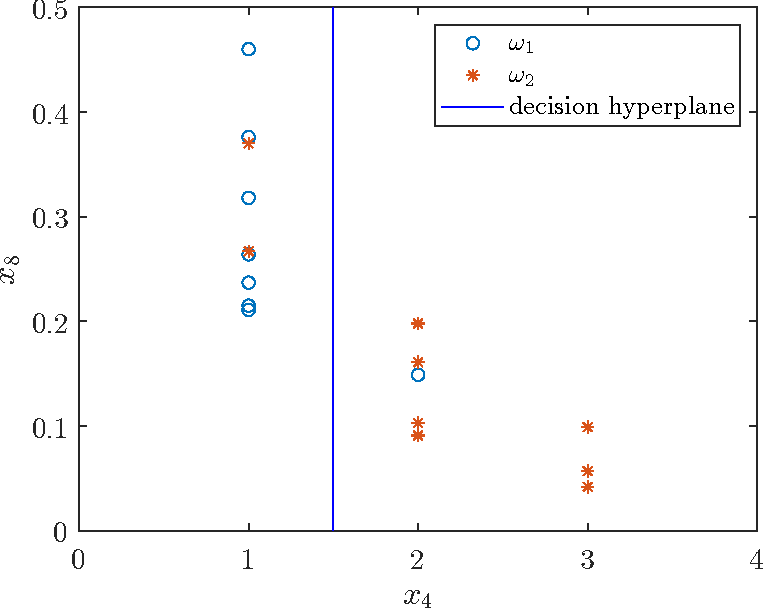
\includegraphics[width=9cm]{featureSVM.pdf}
  \caption{SVM 分类器}
  \label{fig:featureSVM}
\end{figure}

% Reference
\begin{thebibliography}{1}

\bibitem{ReliefF}
Robnik-Šikonja M, Kononenko I. Theoretical and empirical analysis of ReliefF and RReliefF[J]. Machine learning, 2003, 53(1): 23-69.

\bibitem{Relief-based}
Urbanowicz R J, Meeker M, La Cava W, et al. Relief-based feature selection: Introduction and review[J]. Journal of biomedical informatics, 2018, 85: 189-203.

\bibitem{MLbook}
Zhihua Zhou. Machine Learning[J]. 2016. ISBN 978-730-24-2327-8.

\end{thebibliography}

\end{document}
